

\documentclass[12pt,a4paper]{article}\usepackage[]{graphicx}\usepackage[]{color}
%% maxwidth is the original width if it is less than linewidth
%% otherwise use linewidth (to make sure the graphics do not exceed the margin)
\makeatletter
\def\maxwidth{ %
  \ifdim\Gin@nat@width>\linewidth
    \linewidth
  \else
    \Gin@nat@width
  \fi
}
\makeatother

\definecolor{fgcolor}{rgb}{0.345, 0.345, 0.345}
\newcommand{\hlnum}[1]{\textcolor[rgb]{0.686,0.059,0.569}{#1}}%
\newcommand{\hlstr}[1]{\textcolor[rgb]{0.192,0.494,0.8}{#1}}%
\newcommand{\hlcom}[1]{\textcolor[rgb]{0.678,0.584,0.686}{\textit{#1}}}%
\newcommand{\hlopt}[1]{\textcolor[rgb]{0,0,0}{#1}}%
\newcommand{\hlstd}[1]{\textcolor[rgb]{0.345,0.345,0.345}{#1}}%
\newcommand{\hlkwa}[1]{\textcolor[rgb]{0.161,0.373,0.58}{\textbf{#1}}}%
\newcommand{\hlkwb}[1]{\textcolor[rgb]{0.69,0.353,0.396}{#1}}%
\newcommand{\hlkwc}[1]{\textcolor[rgb]{0.333,0.667,0.333}{#1}}%
\newcommand{\hlkwd}[1]{\textcolor[rgb]{0.737,0.353,0.396}{\textbf{#1}}}%
\let\hlipl\hlkwb

\usepackage{framed}
\makeatletter
\newenvironment{kframe}{%
 \def\at@end@of@kframe{}%
 \ifinner\ifhmode%
  \def\at@end@of@kframe{\end{minipage}}%
  \begin{minipage}{\columnwidth}%
 \fi\fi%
 \def\FrameCommand##1{\hskip\@totalleftmargin \hskip-\fboxsep
 \colorbox{shadecolor}{##1}\hskip-\fboxsep
     % There is no \\@totalrightmargin, so:
     \hskip-\linewidth \hskip-\@totalleftmargin \hskip\columnwidth}%
 \MakeFramed {\advance\hsize-\width
   \@totalleftmargin\z@ \linewidth\hsize
   \@setminipage}}%
 {\par\unskip\endMakeFramed%
 \at@end@of@kframe}
\makeatother

\definecolor{shadecolor}{rgb}{.97, .97, .97}
\definecolor{messagecolor}{rgb}{0, 0, 0}
\definecolor{warningcolor}{rgb}{1, 0, 1}
\definecolor{errorcolor}{rgb}{1, 0, 0}
\newenvironment{knitrout}{}{} % an empty environment to be redefined in TeX

\usepackage{alltt}
\usepackage{amsmath}
\usepackage{enumerate}
\usepackage[cm]{fullpage}
\usepackage{graphicx}
\IfFileExists{upquote.sty}{\usepackage{upquote}}{}
\begin{document}
\setlength\parindent{0cm}
%\setlength{\oddsidemargin}{0.25cm}
%\setlength{\evensidemargin}{0.25cm}
\title{\Large{\textbf{Introduction to \texttt{R}}}\\
\textit{Session 5 exercises}}
\author{Statistical Consulting Centre}
\date{2 March, 2017}
\maketitle
 
 

\section{Boxplots}
\label{sec:box}
Produce a boxplot showing the distribution of nerdy scores for each age group as shown in Figure \ref{fig:box1}.
\begin{figure}[h]   
 \centering
\begin{knitrout}
\definecolor{shadecolor}{rgb}{0.969, 0.969, 0.969}\color{fgcolor}
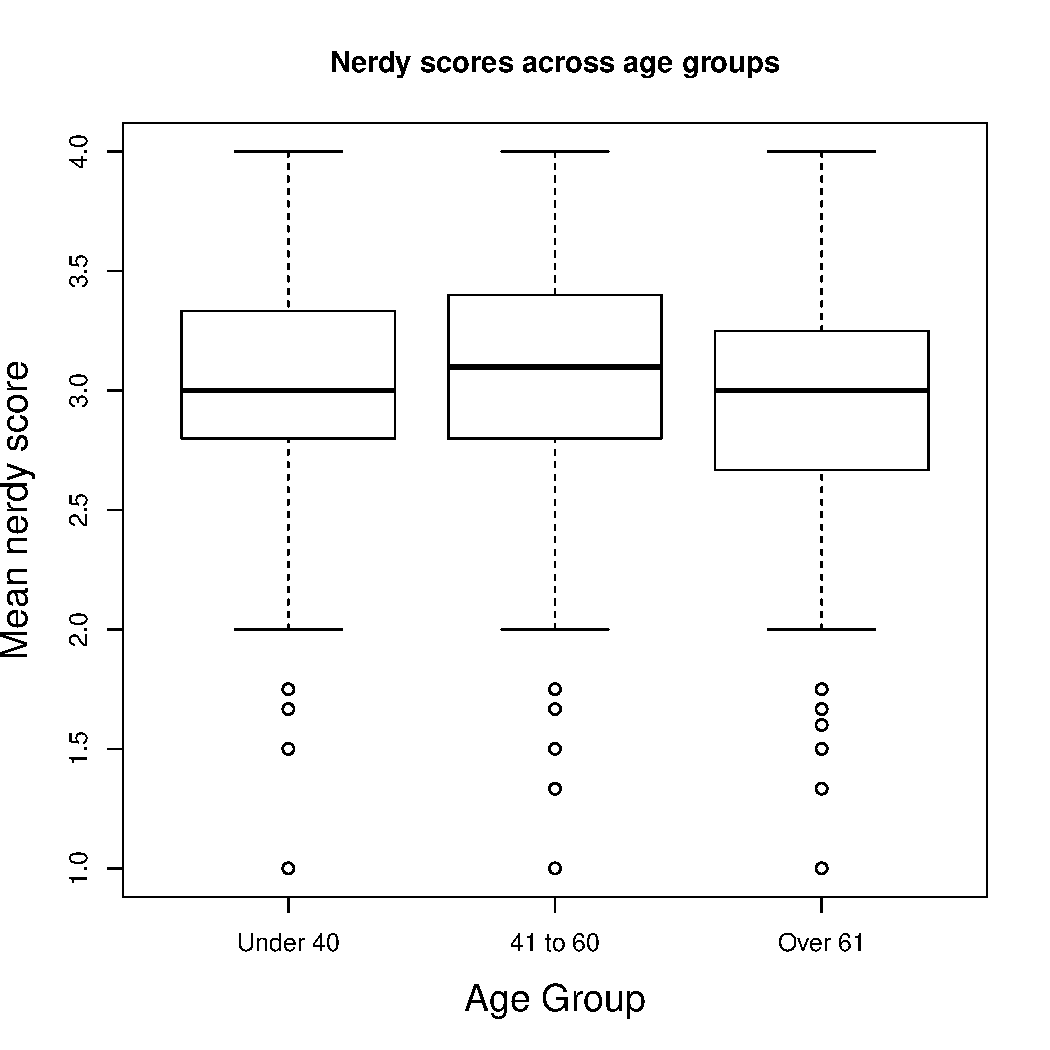
\includegraphics[width=0.7\textwidth]{figure/box1-1} 

\end{knitrout}
\caption{Boxplot in \ref{sec:box}}
  \label{fig:box1}
\end{figure}\\
The graph should have:
\begin{itemize}
\item labels for x and y axes that are large enough to read.
\item a title.
\end{itemize}

\section{Barplots}
\label{sec:bar}
Produce the barplot, shown in Figure \ref{fig:bar1}, based on the information contained in the following table.
\begin{knitrout}
\definecolor{shadecolor}{rgb}{0.969, 0.969, 0.969}\color{fgcolor}\begin{kframe}
\begin{alltt}
\hlstd{q1c.gender.tab} \hlkwb{<-} \hlkwd{with}\hlstd{(sports.df,} \hlkwd{round}\hlstd{(}\hlkwd{prop.table}\hlstd{(}\hlkwd{table}\hlstd{(q1c, gender),} \hlnum{2}\hlstd{)}\hlopt{*}\hlnum{100}\hlstd{,} \hlnum{1}\hlstd{))}
\hlstd{q1c.gender.tab}
\end{alltt}
\begin{verbatim}
                                    gender
q1c                                  Female Male
  Daily                                 4.1  3.2
  Several times a week                 36.1 21.5
  Several times a month                43.9 49.2
  Several times a year or less often   15.9 26.1
\end{verbatim}
\end{kframe}
\end{knitrout}
\begin{figure}[h]   
 \centering
\begin{knitrout}
\definecolor{shadecolor}{rgb}{0.969, 0.969, 0.969}\color{fgcolor}
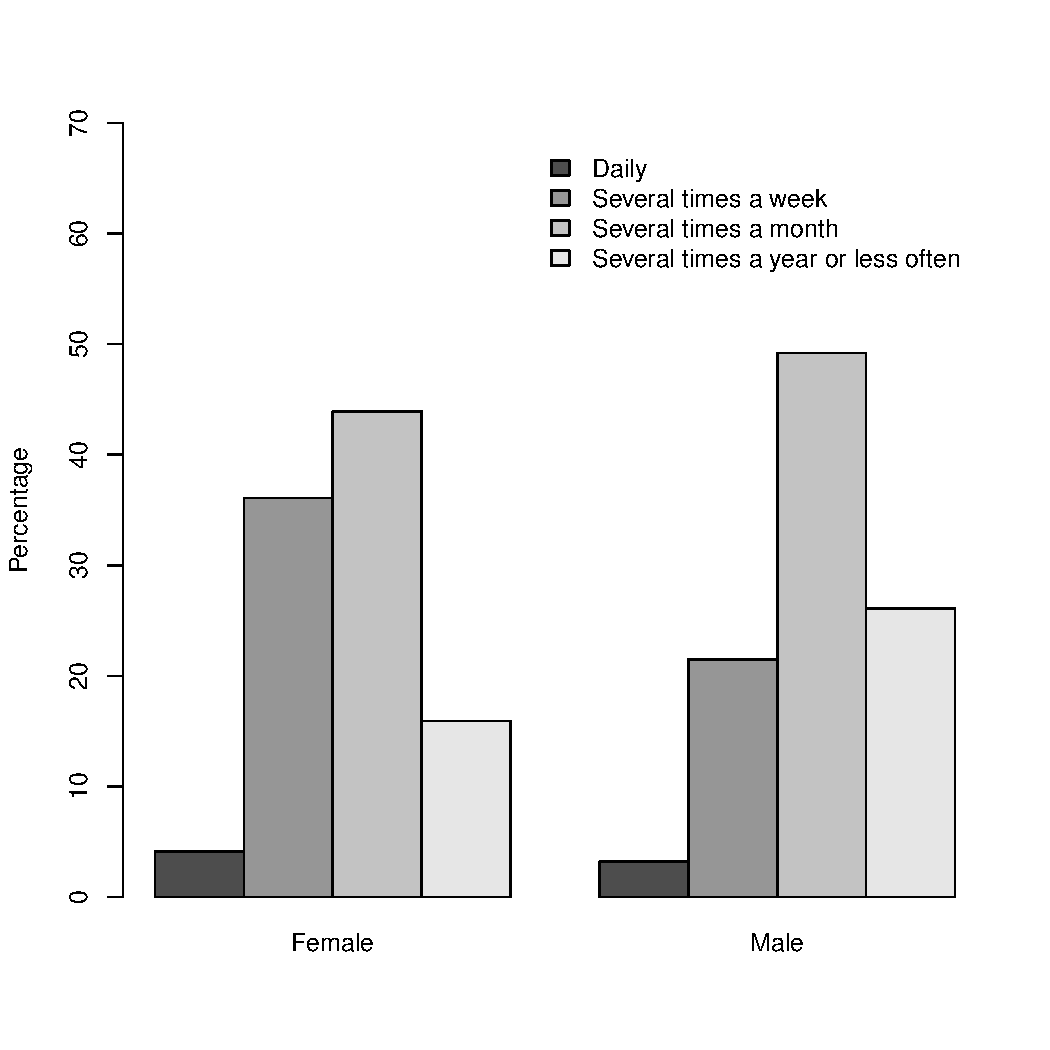
\includegraphics[width=0.7\textwidth]{figure/bar1-1} 

\end{knitrout}
\caption{Barplot in \ref{sec:bar}}
  \label{fig:bar1}
\end{figure}
The graph should contain suitable:
\begin{itemize}
\item axis labels and
\item legend.
\end{itemize}
\end{document}
